\documentclass{beamer}

\usepackage{comment}
\usepackage{tabularx}
\usepackage{bm}

\def\imagetop#1{\vtop{\null\hbox{#1}}}

\def \lecturetitle {Course-specific Search Engines: Semi-automated Methods for Identifying High Quality Topic-specific Corpora}
\def \slidestring {\insertframenumber}

\setbeamercolor{alerted text}{fg=gray}
\author{Neel Guha, Matt Wytock \\ Gunn High School, Carnegie Mellon University}
\usepackage{hyperref}
\usepackage{amsmath}
\usepackage{amssymb}
\usepackage{fancybox}
\usepackage{fancyvrb}
\usepackage{xcolor}
\usepackage{amsthm}
\usepackage{graphicx}
\usepackage{multirow}
\usepackage{gensymb}

%\usepackage{tcolorbox}


\definecolor{lightblue}{rgb}{.161,.502,.725}

\setbeamercolor{normal text}{fg=white,bg=black}
\setbeamercolor{item}{parent={local}}
\setbeamercolor{alerted text}{fg=red}

\setbeamercolor{title}{fg=lightblue}
\setbeamercolor{frametitle}{fg=lightblue}

\usefonttheme[onlymath]{serif}

\setbeamertemplate{navigation symbols}{}
\setbeamertemplate{frametitle}
{
\begin{centering}
\vspace{15pt}
\textbf{\insertframetitle}\par
\end{centering}
}

%\setbeamertemplate{footline}{\hspace{15pt}\tiny{\classnumber: \lecturetitle
%\hfill\insertframenumber}\hspace{15pt} \vspace{15pt}}
%\setbeamertemplate{footline}{\hfill \slidestring\hspace{10pt}\vspace{10pt}}
\setbeamertemplate{}



% small centered block
\newenvironment<>{varblock}[2][\textwidth]{
    \begin{center}
      \begin{minipage}{#1}
      \renewcommand{\'}{\symbol{13}}
        \setlength{\textwidth}{#1}
        \setlength{\leftmargin}{12pt}
          \begin{actionenv}#3
            \def\insertblocktitle{#2}
            \par
            \usebeamertemplate{block begin}
            \begin{semiverbatim}}
  {\par \end{semiverbatim}
      \usebeamertemplate{block end}
    \end{actionenv}
  \end{minipage}
\end{center}}


% itemize seperation
\newlength{\wideitemsep}
\setlength{\wideitemsep}{\itemsep}
\addtolength{\wideitemsep}{12pt}
\let\olditem\item
\renewcommand{\item}{\setlength{\itemsep}{\wideitemsep}\olditem}

\setlength{\leftmargini}{12pt}
%\leftmarginii
%\leftmarginiii


\DeclareMathOperator*{\minimize}{minimize}
\DeclareMathOperator*{\maximize}{maximize}
\DeclareMathOperator*{\subjectto}{subject\;to}
\DeclareMathOperator*{\diag}{diag}

\setbeamertemplate{itemize item}{\hspace{-20pt}$\bullet$}
\setbeamertemplate{itemize subitem}{--}




\title{\textbf{\lecturetitle}}


\begin{document}

\maketitle

\begin{frame}
\frametitle{The educational context}
\begin{itemize}
\item Web search is an important tool for students of all levels
\item In this work, we focus on the high school level and specifically the AP
  United States History (APUSH) course taken by 400,000 students in 2011
\item For these students, there are a number of problems with generic
  keyword-based search engines
\item Goal: Create a search engine specialized to every course
\end{itemize}
\end{frame}

\begin{frame}
\frametitle{Problems with keyword search}
\begin{itemize}
\item {\bf Off-topic results}. [benjamin franklin] brings up plumbing service;
  [gold rush] brings up pages related to Gold Country tourism
\item {\bf Inappropriate sources}. Many sources not reputable, including
  user-generated content (forums, Yahoo answers); sites offering other student
  essays; biased sites (ConfederateAmericanPride.com)
\item {\bf Wrong level}. [thomas jefferson] returns a page from the children's
  version of Library of Congress; typically no explicit labeling for level
\end{itemize}
\end{frame}

\begin{frame}
\frametitle{Google Custom Search Engine}
\begin{itemize}
\item Takes care of difficult task of crawling the web, building an index
  and running a search engine
\item Given a list of sites, can boost these in the results or restrict to just
  these sites (we use restrict in our experiments)
\item Available at \url{http://google.com/cse}
\end{itemize}
\end{frame}

\begin{frame}
\frametitle{APUSH textbook}
\begin{itemize}
\item The American Pageant, Twelfth Edition. (available online)
\item 42 chapters, 1034 pages
\item Authoritative document describing the course
\item Structured information such as chapters, sections, charts, tables, chronology,
  references, etc. (not yet used)
\end{itemize}
\end{frame}

\begin{frame}
\frametitle{APUSH reference search engine}
\begin{itemize}
\item We extracted 1206 distinct proper nouns using syntactic cues (capitalization,
  puctuation, etc.) and took combinations of these to form our query set
\item We issue these queries to Google and extract 23393 sites with 1757
  occurring $>$10 times  
\item Manually curate list of sites (56\% good) and use this to build the APUSH
  CSE 
\end{itemize}
\end{frame}

\begin{frame}
\frametitle{APUSH CSE evaluation}
\begin{itemize}
  \item Blind side-by-side evaluation by domain experts (APUSH teachers)
\end{itemize}
\begin{center}
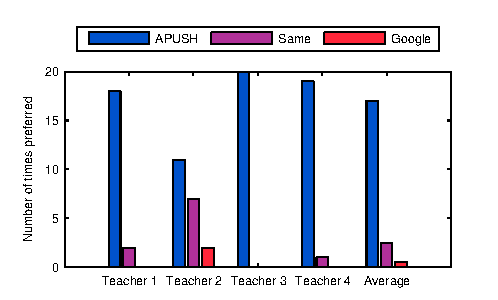
\includegraphics{teacher_eval}
\end{center}
\end{frame}

\begin{frame}
\frametitle{Method 1: TF-IDF weighted text similarity}
\begin{itemize}
\item For each site, concatenate all results from our reference query set
\item Tokenize HTML and stem words using the Porter stemmer
\item Compute TF-IDF weighted cosine distance between the textbook and this synthetic
  document
\end{itemize}
\end{frame}

\begin{frame}
\frametitle{Method 2: Topicality using knowledge bases}
\begin{itemize}
\item Map proper nouns to DBpedia entities using search (``Abe Lincoln'' $\to$ $Abraham\_Lincoln$)
\item DBpedia entities have categories ($Abraham\_Lincoln$
  $\to$ $American\_Presidents$, $Illinois\_Lawyers$,
  $Assassinated\_HeadsOfState$)
\item Form
\begin{equation}
CategoryScore = \frac{\#Textbook}{\#DBpedia}
\end{equation}
where $\#Textbook$, $\#DBpedia$ count number of occurences of an entity 
\item Rank sites according to their category scores
\end{itemize}
\end{frame}

\begin{frame}
\frametitle{Evaluation of automated methods}
\begin{center}
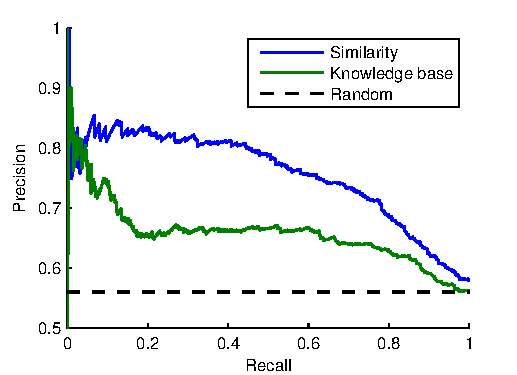
\includegraphics{expt}
\end{center}
\end{frame}

\begin{frame}
\frametitle{Conclusions}
\begin{itemize}
\item Generic search engines with 2-3 word queries cannot fully represent the
  educational context
\item The course textbook provides authoritative text and structured data
\item Future work around how to best utilize this information
\item Current version available at \url{http://guha.com/apushcse.html}
\end{itemize}
\end{frame}

\begin{frame}
\frametitle{Approximating relevance feedback}
\begin{itemize}
\item Reuse manually curated list by randomly selecting 50 good/bad sites (in
  practice this would come from usage logs)
\item Augment textual similarity by
\begin{equation}
RelTextScore = TextScore + GoodScore - BadScore
\end{equation}
where $GoodScore$ and $BadScore$ are textual similarity between the good/bad sites
\item Augment knowledge base scoring by
\begin{equation}
RelCategoryScore = CategoryScore + \#Good + \#Bad 
\end{equation}
where $\#Good$ and $\#Bad$ are the number of good and bad sites associated with
a category.
\end{itemize}
\end{frame}

\begin{frame}
\frametitle{Evaluation with relevance feedback and hybrid scoring}
\begin{center}
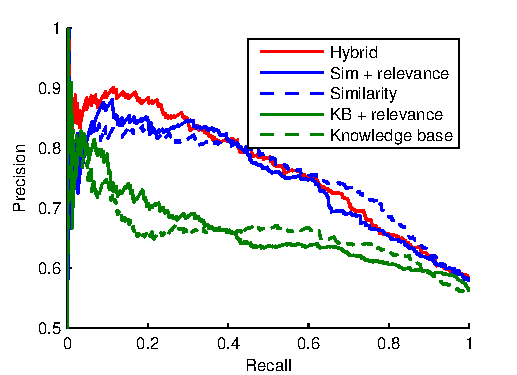
\includegraphics{expt_relevance}
\end{center}
\end{frame}


\end{document}
